\chapter[Introdução]{Introdução}
\label{ch:introdução}
Com o crescente consumo de energia elétrica nos últimos tempos, a demanda por produção da mesma teve um crescimento significativo, trazendo consigo 
impactos ambientais e econômicos. O Brasil por mais que possua em seu território grandes possibilidades para a construção de fontes de obtenção de energia, não
está isento do problema da alta demanda por energia elétrica. Problema que se agravou em 2015 quando o país começou a passar por
uma crise hídrica \cite{crise-hidrica-2015}.

Como a \autoref{fig:rede_convencional} mostra, a maior parte da energia elétrica gerada no Brasil é por meio de hidrelétricas, essa dependência
energética junto com a crise hídrica que o país sofreu culminou em uma política de racionamento e aumento dos impostos - taxa inflacionária no
consumo de energia elétrica - que impactou diretamente a vida de cada cidadão brasileiro, trouxe consequências, como o aumento do 
custo da energia elétrica.

% sustentabilidade


% JONATHAN aqui seu capítulo introdutório. Ele pode conter figuras, tabelas e subseções. Exemplo de uma citação indireta \cite{yu2011new}, e da \autoref{fig:rede_convencional}. Imagens do autor, tem na fonte o texto "Elaborado pelo autor".

\begin{figure}[h!]
	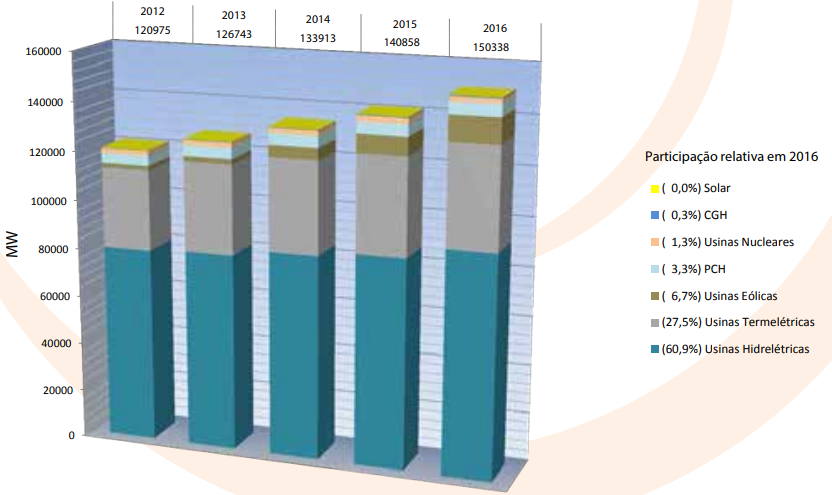
\includegraphics[width=0.9\textwidth, keepaspectratio=true]{forma_energia}
	\centering
	\caption[Capacidade de instalada de geração elétrica no Brasil (MW)]{Capacidade de instalada de geração elétrica no Brasil (MW)}
	\fonte{\cite[p. 57]{epe-anuario}.}
	\label{fig:rede_convencional}
\end{figure}
\FloatBarrier

%%%%%%%%%%%%%%%%%%%%%%%%%%%%%%%%%%%%%%%%%%%%%%%%%%%%%%%%%%%%%%%%%%%%%%%%%%%%%%%%%%%%%%%%%%%%%%%%%%%%%%%%%%%

O Consumo de energia elétrica é um dos principais indicadores de desenvolvimento e de qualidade de vida 
de um país. Esse índice é tão importante que reflete diretamente no ritmo de vida de uma população, pois mostra
se as atividades industriais de uma nação estão ou não em um bom ritmo e pode detectar se o comércio está em alta,
devido aos bens e serviços que o povo adquiriu \cite{energia-desenvolvimento}. Porém um crescimento desordenado na população e um crescimento
exponencial no consumo de energia pode acarretar em problemas para um determinado país.
Analisando os dados \cite{epe-balanco-final}, o consumo de energia  
elétrica no Brasil vem crescendo ao longo dos anos. Segundo \cite{ref-jc}, nos últimos 35 anos teve um crescimento médio de 6,72\%, após a crise que o Brasil sofreu entre os anos 2002 e 2005 houve um crescimento
de 4,91\% na demanda energética do país. A \autoref{fig:consumo_energia_total} retrata o cenário de crise energética que o Brasil vinha
passando ao longo dos anos, até 2008 o país consumia mais do que produzia.

\begin{figure}[h!]
	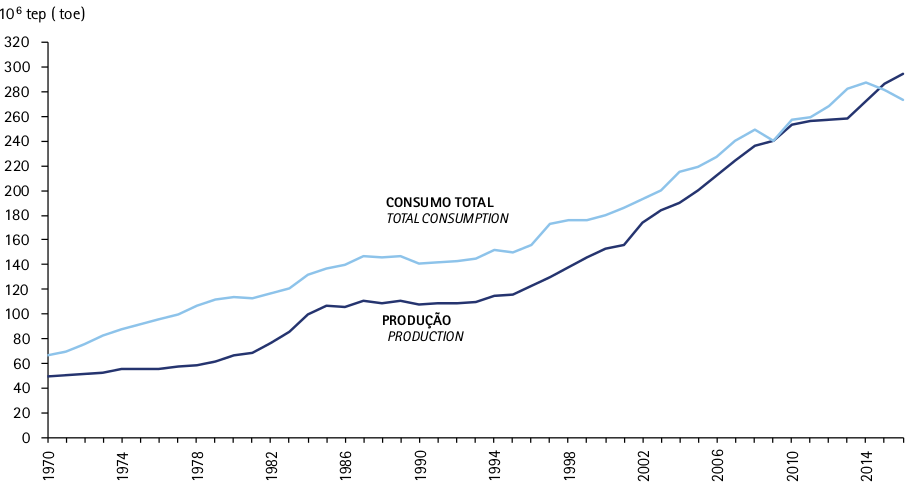
\includegraphics[width=0.85\textwidth, keepaspectratio=true]{consumo_energia_total}
	\centering
	\caption[Estrutura do Consumo de fontes primárias]{Estrutura do Consumo de fontes primárias}
	\fonte{\cite[p. 43]{epe-balanco-final}.}
	\label{fig:consumo_energia_total}
\end{figure}
\FloatBarrier

Para poder acompanhar a crescente demanda por energia elétrica, o governo brasileiro autorizou a contrução de mais de 24 hidrelétricas \cite{governo-preve}.
Um grande problema desse planejamento que o governo fez são os inúmeros impactos ambientais e econômicos, um exemplo prático é a usina de de Belo Monte - Rio Xingu, Pará -. Obra que foi planejada
para ser a maior hidrelétrica do Brasil, com capacidade de abastecer 40\% das residências \cite{energia-abastece}.
Deveria ter sido finalizada completamente e ter seu total funcionamento no segundo semestre de 2015, mas até os dias atuais não opera em 100\%. Vale salientar que a construção
trouxe o desmatamento de áreas indígenas, alagamentos permanentes, comprometimento da fauna e flora e aumento da dificuldade dos transportes fluviais
de comunidades ribeirinhas \cite{ref-g1}.

Diante da problemática do alto consumo de energia elétrica, surge uma indagação: "Construir usinas mesmo sabendo dos impactos negativos que podem surgir, ou não construí-las e
aumentar a tarifação pelo consumo de energia visando um uso mais consciente?". A resposta para essas e outras questões que podem aparecer não são fáceis.
Entretanto o governo brasileiro opitou pela construção de novas usinas e pelo aumento da tarifação no consumo de energia elétrica. 
Uma medida que poderia ser tomada pelo gorverno, seria a chamada "\textit{exposição da informação}". Ao deixar claro 
o quanto o consumidor tem gasto de energia elétrica ao longo do mês, isso acarretaria numa consciêntização do consumo de energia elétrica.

% A evolução da tarifa,
% pode ser observada na \autoref{evolucao-tarifa}


% \begin{table}[!ht]
% 	\centering
% 	\begin{tabular}{lcccc}
% 	\hline
% 	\textbf{Ano} & \multicolumn{1}{l}{\textbf{1º Trimestre}} & \multicolumn{1}{l}{\textbf{2º Trimestre}} & \multicolumn{1}{l}{\textbf{3º Trimestre}} & \multicolumn{1}{l}{\textbf{4º Trimestre}} \\ \hline
% 	\rowcolor[HTML]{DDDDDD} 
% 	2013         & 120,8                                     & 117,1                                     & 114,5                                     & 116,1                                     \\
% 	2014         & 121,1                                     & 127,6                                     & 134,4                                     & 141,9                                     \\
% 	\rowcolor[HTML]{DDDDDD} 
% 	2015         & 154,2                                     & -                                         & -                                         & -                                        
% 	\end{tabular}
% 	\caption{Evoluçao dos custos de energia elétrica em R\$/MWh}
% 	\fonte{\cite[p. 1]{evolucao-tarifa-ref}}
% 	\label{evolucao-tarifa}
% \end{table}

% Uma medida totalmente cabível que ainda é desconhecida por alguns brasileiros é a chamada "\textit{exposição da informação}", deixando sempre bem claro 
% quanto o consumidor tem gastado ou consumindo ao longo do mês em sua residência, isso é possível graças a equipamentos que estão sempre monitorando
% a rede elétrica.Segundo uma pesquisa realizada pela Associação Brasileira das Empresas de Serviços de Conservação de Energia, em seis anos o Brasil 
% desperdiçou o equivalente a 250GWh em energia o que equivale a R\$62 bilhões, desperdício que se deu justamente a tamanha falta de infomação que 
% o consumidor tem, se ao saber o quanto tem consumido ou gastado em tempo real o consumidor poderia se prevenir dos desperdícios. 


% Ao passar dos anos o Brasil vem mostrando cada vez mais o seu potencial na produção de energia, o território brasileiro possibilita as várias formas
% de obtenção da eletricidade. Analisando os dados \cite[p.29]{epe-anuario-2015} e comparando com a \autoref{cap_ele} nota-se que o Brasil subiu duas
% posições no \textit{Rank} de geração de energia elétrica, isso é reflexo do aumentou da capacidade de produção de energia que chegou na marca de 8,39\%.

% \begin{table}[!ht]
% 	\centering
% 	\begin{tabular}{lccccc}
% 		\rowcolor[HTML]{9B9B9B} 
% 		\multicolumn{1}{c}{\cellcolor[HTML]{9B9B9B}} & {\color[HTML]{FFFFFF} \textbf{2010}} & {\color[HTML]{FFFFFF} \textbf{2011}} & {\color[HTML]{FFFFFF} \textbf{2012}} & {\color[HTML]{FFFFFF} \textbf{2013}} & \multicolumn{1}{l}{\cellcolor[HTML]{9B9B9B}{\color[HTML]{FFFFFF} \textbf{2014}}} \\ \hline
% 		\textbf{Mundo}                               & \multicolumn{1}{l}{\textbf{5080,6}}  & \multicolumn{1}{l}{\textbf{5305,0}}  & \multicolumn{1}{l}{\textbf{5514,6}}  & \multicolumn{1}{l}{\textbf{5736,2}}  & \multicolumn{1}{l}{\textbf{6038,7}}                                              \\ \hline
% 		\rowcolor[HTML]{DDDDDD} 
% 		China                                        & 971,8                                & 1069,5                               & 1154,6                               & 1267,7                               & 1399,5                                                                           \\
% 		Estados Unidos                               & 1039,1                               & 1051,3                               & 1063,0                               & 1060,1                               & 1074,6                                                                           \\
% 		\rowcolor[HTML]{DDDDDD} 
% 		Japão                                        & 284,9                                & 287,3                                & 293,3                                & 300,8                                & 313,4                                                                            \\
% 		Índia                                        & 213,1                                & 246,0                                & 260,3                                & 283,0                                & 310,8                                                                            \\
% 		\rowcolor[HTML]{DDDDDD} 
% 		Rússia                                       & 228,1                                & 231,6                                & 233,6                                & 235,2                                & 247,6                                                                            \\
% 		Alemanha                                     & 162,7                                & 167,5                                & 177,3                                & 186,1                                & 198,4                                                                            \\
% 		\rowcolor[HTML]{DDDDDD} 
% 		Canadá                                       & 132,3                                & 132,9                                & 130,7                                & 133,3                                & 136,8                                                                            \\
% 		Brasil                                       & 11,3                                 & 117,1                                & 121,0                                & 126,7                                & 133,9                                                                           
% 	\end{tabular}
% 	\caption{Capacidade instalada de geração elétrica no mundo, 2014 (GW)}
% 	\fonte{\cite[p. 29]{epe-anuario}}
% 	\label{cap_ele}
% \end{table}

% A maior produção de energia do Brasil provem das hidrelétricas, o país é referência mundial quando o assunto é obtenção de energia através de
% usinas hidrelétricas - \autoref{cap_hidro} - isso é possível devido a sua alta concentração de rios de grande porte e ao grande volume de chuva
% que alimenta e reforça o poderio hídrico do país. A energia que a usina hidrelétrica fornece é conseguida através da energia hidráulica que provém
% do aproveitamento da força potencial e cinética das correntes de água,rio, mar. A água ao passar por tubulações com muita força e velocidade 
% movimenta-se as turbinas fazendo com que elas girem em um velocidade suficiente para que os geradores acoplados nas turbinas, transformem energia
% mecânica em energia elétrica, lembrando que a eficiência energética de uma usina hidrelétrica é de 65,2\%. Após esse longo processo a energia 
% extraída é enviada para estações de tratamento e após essa etapa é enviada para a matriz energética que fará a distribuição da energia extraída. 

% \begin{table}[!ht]
% 	\centering
% 	\begin{tabular}{lccccl}
% 		\rowcolor[HTML]{9B9B9B} 
% 		\multicolumn{1}{c}{\cellcolor[HTML]{9B9B9B}} & {\color[HTML]{FFFFFF} \textbf{2010}} & {\color[HTML]{FFFFFF} \textbf{2011}} & {\color[HTML]{FFFFFF} \textbf{2012}} & {\color[HTML]{FFFFFF} \textbf{2013}} & {\color[HTML]{FFFFFF} \textbf{2014}} \\ \hline
% 		\textbf{Mundo}                               & \multicolumn{1}{l}{\textbf{903,9}}   & \multicolumn{1}{l}{\textbf{929,9}}   & \multicolumn{1}{l}{\textbf{957,5}}   & \multicolumn{1}{l}{\textbf{1000,4}}  & \textbf{1038,3}                      \\ \hline
% 		\rowcolor[HTML]{DDDDDD} 
% 		China                                        & 199,5                                & 214,6                                & 229,1                                & 258,9                                & 283,0                                \\
% 		Brasil                                       & 80,7                                 & 82,5                                 & 84,3                                 & 86,0                                 & 89,2                                 \\
% 		\rowcolor[HTML]{DDDDDD} 
% 		Estados Unidos                               & 78,8                                 & 78,7                                 & 78,7                                 & 79,2                                 & 79,7                                 \\
% 		Canadá                                       & \multicolumn{1}{l}{74,9}             & \multicolumn{1}{l}{75,4}             & \multicolumn{1}{l}{75,4}             & \multicolumn{1}{l}{75,4}             & 75,4                                
% 	\end{tabular}
% 	\caption{Capacidade instalada de geração hidrelétrica no mundo, 2014 (GW)}
% 	\fonte{\cite[p. 30]{epe-anuario}}
% 	\label{cap_hidro}
% \end{table}

% É do conhecimento de qualquer brasileiro que possua uma noção básica de geografia que a região norte é a região que possui a maior quantidade de rios,
% essa noção pode levar uma conclusão errada - A região norte é a que mais produz energia - pois nem todo rio tem potencial para que uma hidrelétrica se instale.
% Por sua vez as regiões sul e sudeste são as que mais necessitam de energia, devido a densidade populacional e a quantidade de industrias instaladas nas regiões.
% A \autoref{pxcxge} externa essa problemática de uma maneira bem visível. Percebe-se que por exemplo a região sudeste é a que produz mais energia, porém é a que mais
% gasta, sendo os gastos maiores do que os ganhos, já a região norte e nordeste são regiões que produzem mais do que gastam. Vendo esse total desequilíbrio
% de geração e consumo de energia, surgiu a necessidade da criação do Sistema Interligado Nacional (SIN). O SIN é constituído por todas as regiões brasileiras
% e é interconectado por meio de uma malha de transmissão que propicia a transferência de energia entres os subsistemas, permitindo a obtenção de ganhos
% sinérgicos e explora a diversidade entre os regimes hidrológicos e das bacias. A integração dos recursos de geração e transmissão permite o atendimento ao
% mercado com segurança e economicidade.
% \begin{table}[!ht]
% 	\centering
% 	\begin{tabular}{cccc}
% 		\hline
% 	\textbf{Região} & \textbf{População} & \textbf{Consumo em GW} & \textbf{\begin{tabular}[c]{@{}c@{}}Capacidade Instalada de \\ Geração Elétrica GW\end{tabular}} \\ \hline
% 		\rowcolor[HTML]{DDDDDD} 
% 		Norte           & 17.707.783         & 12,197                 & 25,484                                                                                          \\
% 		Nordeste        & 56.915.936         & 12,109                 & 29,803                                                                                          \\
% 		\rowcolor[HTML]{DDDDDD} 
% 		Sudeste         & 86.356.952         & 74,584                 & 44,810                                                                                          \\
% 		Sul             & 29.439.773         & 19,173                 & 31,681                                                                                          \\
% 		\rowcolor[HTML]{DDDDDD} 
% 		Centro-Oeste    & 15.660.988         & 5,634                  & 18,558                                                                                         
% 	\end{tabular}
% 	\caption{Relação População x Consumo por Região x Geração Elétrica por Região}
% 	\fonte{(IBGE\protect\footnotemark  e  EPE\protect\footnotemark)}
% 	\label{pxcxge}
% \end{table}

% \addtocounter{footnote}{-1}
% \footnotetext{\cite{epe-balanco-final}}
% \addtocounter{footnote}{1}
% \footnotetext{\url{https://ww2.ibge.gov.br/home/estatistica/populacao/estimativa2009/estimativa.shtm}{}}


% Após entender todo o funcionamento da geração e distribuição de energia no Brasil, é conveniente entender o processo de leitura do consumo de 
% energia elétrica.

% Os primeiros medidores de eletricidade foram utilizados na operação de lâmpadas em série, um vez que a tensão era constante, a corrente exigida
% por cada lâmpada era conhecida e todas estavam ligadas no mesmo interruptor, os medidores foram suficientes apenas para medir o gasto das lâmpadas
% em um tempo determinado, surgindo o termo - lâmpada-hora. Em 1872 o pesquisador Samuel Gardiner trouxe a toda a primeira patente sobre um contator 
% de energia, que era formado por uma lâmpada acoplada a um contador de energia DC controlado por um relógio e um eletroímã, ao passar do tempo várias
% outras patentes foram surgindo e tentando melhorar o projeto de Samuel Gardiner, mas foi apenas em 1892 que que surgiu o primeiro medidor de watt-hora
% com precisão e confiabilidade suficiente para aplicação em medição de consumo de energia. Criado por Thomas Duncan, inicialmente seu objetivo era a medição
% de circuitos monofásicos, porém com o bom desempenho do aparelho modificações foram feitas para à medição de circuitos polifásicos de energia.

% Atualmente a energia elétrica é quantificada através de um equipamento chamado medidor, que nos dias atuais a medição é feita em quilowatt-hora.
% Os medidores da atualidade são caracterizados por padrões da norma NBR 14519, o grupo de medidor mais utilizado pelas concessionárias nas residências
% é o grupo B. 

% \begin{itemize}
% 	\item Grupo B \\
% 	É caracterizado por unidades consumidoras de baixa tensão, com tensões inferiores a 2,3KV. As unidades consumidores podem ser classificadas
% 	mediante a necessidade da concessionária responsável, geralmente o tipo B1 é residencial, tipo B2 são as residências rurais e estabelecimentos
% 	comerciais ou industriais são classificados como o tipo B3.
% \end{itemize}

% Estima-se que 92\% dos medidores em funcionamento são eletromecânicos, pois são de baixa custo e de boa qualidade, com o erro máximo de 2\% de seu valor
% nominal de operação. Não ter um medidor em uma unidade consumidora pode gerar transtornos tanto para concessionário, pois não saberá o quanto deve cobrar ao 
% consumidor, como para o dono do estabelecimento, pois não terá o aporte devido prestado pela concessionária de energia.


% Mesmo com a grande evolução que os medidores eletromecânicos sofreram ao longo do tempo, os dispositivos ainda apresentam pontos frágeis, dando uma 
% grande margem ao erro. A grande quantidade de peças mecânicas presente no medidor, faz com que o mesmo possua algumas limitações: interferência na
% opereção na presença de corrente continua que causam deformações no fluxo magnético do leitor; diminuição da precisão quando são tratados de valores
% muito baixos. Hoje em dia existe uma forte tendência a substituição desses medidores eletromecânicos por medidores eletrônicos. A troca irá possibilitar além de uma
% melhor precisão, uma maior e melhor medição e até possibilitando uma leitura remota. Hoje no Brasil existe um projeto de lei (PL 2932/20015) que prevê
% a substituição de medidores de consumo de energia eletromecânicos por medidores eletromecânicos inteligentes em até 15 anos após a aprovação da lei.

% %%%%%%%%%%%%%%%%%%%%%%%%%%%%%%%%%%%%%%%%%%%%%%%%%%%%%%%%%%%%%%%%%%%%%%%%%%%%%%%%%%%%%%%%%%%%%%%%%%%%%%%%%%%%

% A necessidade de contornar os desafios da crescente demanda energética incentiva a busca por fontes alternativas e limpas de energia. A \autoref{fig:fonte_energia} mostra
% que o Brasil vem investindo ao passar dos anos em fontes limpas de energias. Analisando os dados da imagem é possível notar na imagem que não basta apenas ter fontes limpas
% e renováveis de energia, é necessário buscar melhorias como as Smart Grids.

% \begin{figure}[h!]
% 	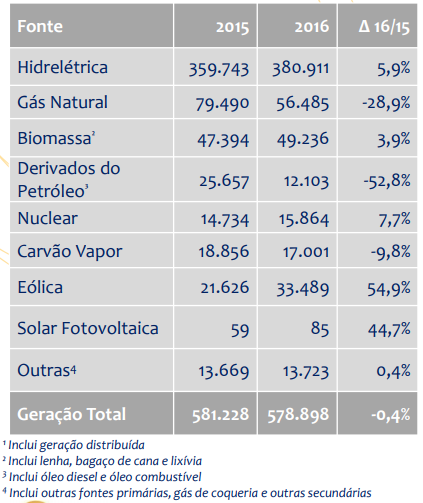
\includegraphics[width=0.7\textwidth, keepaspectratio=true]{fontes_energia}
% 	\centering
% 	\caption[Fontes de geração de energia elétrica (GWh)]{Fontes de geração de energia elétrica (GWh)}
% 	\fonte{\cite[p. 35]{epe-balanco}.}
% 	\label{fig:fonte_energia}
% \end{figure}
% \FloatBarrier

% As chamadas redes inteligentes de transmissão e distribuição de energia, \textit{smart grid}, tem como objetivo conectar unidades descentralizadas de geração
% grande e pequena com o consumidor final. Assim nessa ideia o fluxo de energia se comunica de uma maneira bidirecional, a energia que é tradicionalmente
% gerada e distribuida pelas concessionárias poderá ser gerada e integrada as redes elétricas a partir de unidades consumidoras. O grande pilar dessa 
% tecnologia são os sensores instalados ao longo da rede elétrica que constantemente estão enviando informações referente ao consumo a concessionária,
% possibilitando um planejamento mais eficiente da rede. Aliado aos sensores na rede elétrica o consumidor recebe um medidor inteligente que também
% é integrado com a concessionária em tempo real.

% \begin{figure}[h!]
% 	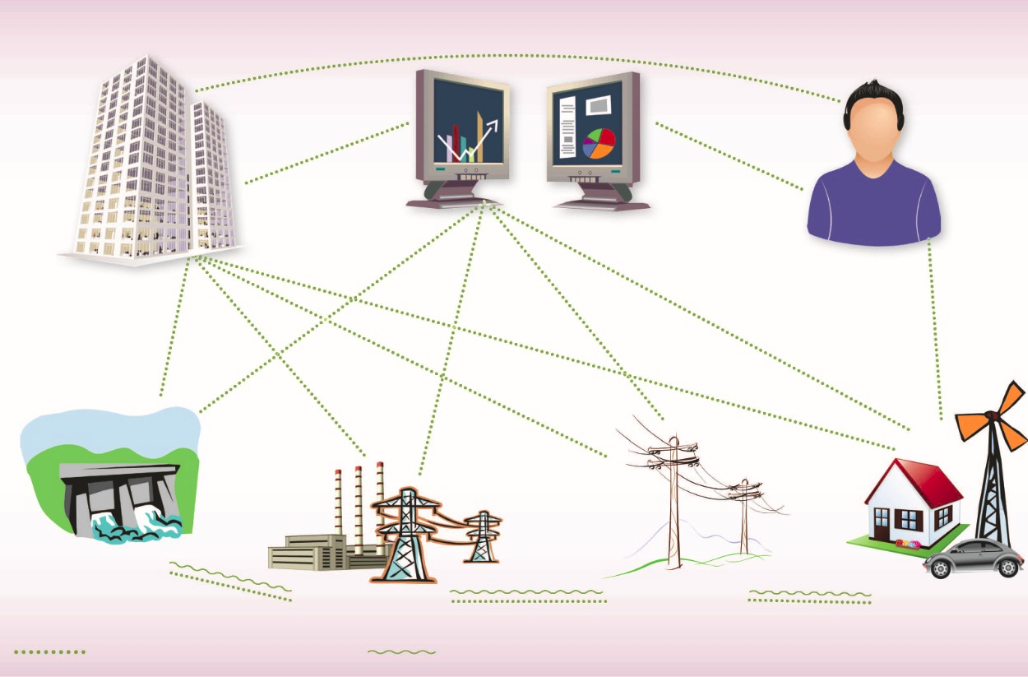
\includegraphics[width=0.7\textwidth, keepaspectratio=true]{rede_smartgrid}
% 	\centering
% 	\caption[Smart Grid,comunicação inteligente entre todos os usuários]{Smart Grid,comunicação inteligente entre todos os usuários}
% 	\fonte{\cite{smart-grid}.}
% 	\label{fig:rede_smartgrid}
% \end{figure}
% \FloatBarrier

O trabalho apresentará uma forma barata e eficiente de monitorar a energia elétrica de uma residência em tempo real, disponibilizando informações valiosas ao usuário.
O sistema também disponibiliza de ferramentas para que 
caso o usuário possua o conhecimento necessário o mesmo venha a modificar ou aprimorar o gerenciamento de energia. O sistema nomeado de \textit{Power Monitor}
traz consigo uma nova forma de enxergar o consumo dos aparelhos presentes em uma residência, trocando o quilowatt-hora pela moeda de circulação no país,
o real, tal mudança é o principal fator de conscientização, pois aproxima o consumidor dos gastos energéticos.


\section{Motivação}

A motivação deste trabalho partiu da analise da atual conjuntura do cenário energético brasileiro que é baseado na falta de transparência da 
informação levada ao usuário \cite{ref-conju}. Notando-se a dificuldade de entender o consumo de energia elétrica dos dispositivos presentes em uma 
residencia, fez-se necessário o desenvolvimento de um sistema de monitoramento para uso consciente da energia elétrica.
% ter informação em tempo real do consumo de energia em um estabelecimento é muito difícil, pois os equipamentos que proporcionam esse tipo de informação
% não são acessíveis a todos os brasileiros, apenas companhias de energia ou pessoas com alto grau de estudo conseguem manusear ou entender o dados
% fornecidos por esse tipo de equipamento. Toda essa privação da informação traz consequências, uma delas é o descaso do brasileiro em relação ao
% racionamento de energia elétrica, como já foi citado no trabalho o Brasil em seis anos desperdiçou o equivalente a R\$ 62 bilhões, motivo que se 
% dá a falta de conscientização do consumidor. Trazer uma forma com que consumo de energia elétrica, conta de luz, fique mais fácil e simples de se entender
% e acompanhar é o que o sistema \textit{power monitor} fará.   

\section{Objetivos}
O objetivo deste trabalho é propor um sistema de monitoramento de energia elétrica, de baixo custo, para o uso consciente da mesma. 
O sistema faz uso de medições e cálculos para uma melhor visualização do consumo de energia. Onde o seu principal diferencial é a troca da unidade de medida 
referente ao consumo elétrico de um aparelho pela moeda de circulação no pais.

% O \textit{Power Monitor} é um sistema de computador composto por um servidor \textit{web} e uma interface \textit{web} de fácil comunicação com \textit{hardwares} que possam 
% se conectar a uma rede \textit{Wi-Fi}. O sistema é baseado na obtenção dos dados que são aferidos através do sensor de corrente.  

% A objetivo existente neste trabalho é da conscientização do consumidor em relação aos gastos energéticos presentes em sua residência. Percebendo o
% atual cenário brasileiro de total falta de informação em relação ao consumo em tempo real de energia, junto com o período em que o país 
% passou de crise hídrica e energética, este trabalho propõe uma alternativa simples e barata onde qualquer brasileiro independente do grau de 
% escolaridade ou classe social poderá acompanhar o consumo de energia elétrica de sua residência de uma maneira mais fácil e direta. O \textit{power monitor}
% é composto por elementos de \textit{software} e \textit{hardware} que gerenciam automaticamente todos os dispositivos cadastrados presentes em uma
% residência, esse gerenciamento se deve ao conjunto formado pelo servidor \textit{web} que é responsável por enviar e receber informações ao \textit{hardware} e
% a interface \textit{web}, juntamento com o banco de dados que é responsável por guardar todas as informações coletadas pelo \textit{hardware} e a interface
% \textit{web} tem o papel de agente consumidor de todos os dados e tratará as informações da melhor forma possível.


\section{Metodologia}
O Power Monitor foi implementado utilizando a linguagem de programação JavaScript que por sua vez se comunica com uma placa de desenvolvimento NodeMCU. 
O Power Monitor possui um servidor web que é responsável por gravar todos os dados coletados em um banco de dados e fazer a comunicação entre softaware e Hardware. 
A interface web consome todos os dados gravados e após trata-los e realizar alguns cálculos o resultado é apresentado em forma de gráficos e alertas.

\section{Levantamento bibliográfico}
Trabalhos relacionados ao monitoramento de energia residencial têm sido mais comuns nos últimos anos. Como o monitoramento pode ser feito utilizando eletrônicos e comunicação
sem fio, os diversos trabalhos tem se direcionado a desenvolver sistemas utilizando microcontroladores e sensores.


\cite{ref-jlgb} foi desenvolvido com base na implementação de um sistema particular de monitoramento de consumo de energia elétrica, em tempo real e não invasivo.
Com o auxílio da plataforma de prototipagem Arduino e dos sensores de corrente e tensão é possível monitorar em tempo real o consumo de uma residência. O intuito principal
desse trabalho é a conscientização pela economia de energia.

O \cite{ref-apc} é um protótipo desenvolvido para ser um sistema de medição de consumo de energia elétrica no setor residencial, onde os valores de medição
apresentados para o usuário são convertidos para valores monetários.


O trabalho \cite{ref-rpc} visa o monitoramento de energia elétrica, desenvolvido para se comunicar com um sistema \textit{web} e com um aplicativo de celular.
Com o objetico de usar as informações coletadas pelo dispositivo \textit{Powersave} e disponibilizar ao usuário, para que assim poassa conscientezar o consumo de energia elétrica.

\section{Estrutura do Trabalho}
O trabalho foi estruturado para que se possa mostrar nos próximos capítulos os seguintes conteúdos:
\begin{itemize}
	\item Capítulo 2: Embasamento Teórico - Descrição das tecnologias utilizadas neste trabalho;
	\item Capítulo 3: Desenvolvimento - Será descrita as etapas de implementação do projeto, desde uma visão geral do funcionamento a comunicação entre \textit{hardware} e servidor \textit{web};
	\item Capítulo 4: Conclusão - Conclusão e trabalhos futuros;
\end{itemize}